\documentclass{article}
\usepackage{enumitem}
\usepackage{graphicx}
\usepackage{grffile}
\usepackage{float}
\begin{document}
\title{%
 Deliverable 1\\
 \large An identification of problems, derivation of high level requirements\\
 \large and an articulation of features using controlled notation
}
\author{Epic Group}
\date{}
\maketitle

\section*{Introduction}
The purpose of this report is to identify and express high level requirements
regarding a potential software system via structured notation. We will express
the contents of our report in the following format.
\begin{enumerate}
\item \textbf{Problem Statements}: A series of problem statements which will
investigate a number of problems we will solve via our software prototype.
\item \textbf{User Stories}: An idenfitication of features based on the problem
statement previously specified.
\item \textbf{Low-Fidelity Prototype}: A paper physical sketch of the UI 
elements integrated with a storyboard-like chronological script.
\item \textbf{High-Fidelity Prototype}: A computerised render of the
low-fidelity prototype previously specified.
\end{enumerate}
Our report will strictly harbor to controlled software engineering notation, 
such as the utilisation of user stories and Connextra notation.
\section{Problem Statements}
We will enumerate over a series of problem statements, tangibly solved by
software, potentially resolved in our prototype. Subsequently, we will choose
to target a specific problem statement within the remainder of our report.
\subsection{Media Recommendations Problem Statement}
Recommendations of visual media on contemporary popular internet platforms are
inaccurate, biased or limited. Recommendation algorithms on such platforms are
often a small subsection of a larger media streaming or distribution service, 
restricting the scope of recommendation to those within such a service. Moreover, 
recommendation systems are typically implemented with small data sets and cheap 
computational cost as a priority. As a result, recommendations provided to a 
user are fragmented, unreliable and erroneous.
\subsection{Internet Misinformation Problem Statement}
Information presented by news media outlets and online sources of information
can frequently be misleading or malicious. In addition, the advent of social
media platforms permitting and stimulating the concept of sudden, mass 
popularity has encouraged the threat of misinformation spreading routinely and
to great negitive effect. In response, the employment of paid moderators have
only further exacerbated the issue, with themselves enforcing their baiases
regarding which information is legal.
\subsection{Credential Security Problem Statement}
Due to the prevalence of database leaks combined with the tendency of internet
users to share credentials across multiple platforms, identities on the internet
are frequently hijacked. Moreover, specific individuals are often targeted in
order to spread disinformation and aid in monentary theft. Current database
credential storage technologies are inadquate in reducing user harm during the
seemingly inevitable event that a webserver security solution is bypassed.
\subsection*{Chosen Problem Statement}
We have decided to focus our attention towards developing a software prototype
which solves the media recommendations problem statement. The alternative 
problem statements are difficult to target in the small timeframe we have been
provided. In contrast, a solution to the media recommendation problem statement 
is relatively managable to implement. Moreover, it also fulfills the requirement
of communicating with an information archive via an API
(application programming interface).

\iffalse

1.The Search result of movies with keywords are fragmented, less related and inaccuracy.

2.The website pages are mess and unreadable.

3.Searching movies with multiple tags is unfriendly and the operation is complicated.

\fi


\section{Features and User Stories}
We will initially decompose our chosen problem statement into a set of high
level requirements. Our high level requirements will then be further classified
into a set of features. We will utilise Connextra notation when describing
each feature, concluding by elicitating a set of user stories that accurately
describe our feature set.
\subsection{High Level Requirements and Features}
\begin{enumerate}
\item
\textbf{High Level Requirement}: A device agnostic web based user interface.
\newline
\textbf{Feature}: A lightweight HTML (Hyper Text Markup Language) and Javascript
based user interface utilising the open source Bulma CSS (Cascading Style Sheets)
stylesheet.
\item 
\textbf{High Level Requirement}: A media recommendation system.\newline
\textbf{Feature}: A procedurally generated series of questions which narrows
down a set of recommended movies based on the previous response.
\item 
\textbf{High Level Requirement}: Information about specific media. \newline
\textbf{Feature}: Requests to the IMDb (Internet Movie Database) and OMDB
(Open Movie Database) retrieving the title, rating and description of movies,
among others.
\item
\textbf{High Level Requirement}: A performant webserver stack capable of fast
responses under a heavy workload per user session.\newline
\textbf{Feature}: The use of a compiled, high performance programming language
along with the Pistache HTTP and REST (Representational State Transfer)
framework.
\item
\textbf{High Level Requirement}: Reliability and maintainability for any 
software written ensuring user frontend stability.\newline
\textbf{Feature}:
The use of the GoogleTest C++ testing framework, javascript and HTML linters
along with continuous integration testing.
\end{enumerate}
\subsection{User Stories}
The following user stories are symbolically linked to the aforementioned high
level requirments and features.
\begin{itemize}
\item
\textbf{Mobile User}: As a user of multiple devices, each with their own set
of human interface devices, I want to be able to access the website through
either device. Given that I am using a mobile phone or desktop, I wish to
be able to receive movie recommendations regardless of my choice of device.

\item
\textbf{Media Recommendation System}: As an avid film consumer, I want to
receive tailored, specific recommendations relevant to me. Given that I am
visiting the website, I wish to be able to discover esoteric and popular
films alike without being limited to a biased or limited database.

\item
\textbf{Media Information}: As a selective film consumer, I wish to cherry pick
a movie based on specific details such as film rating, length and content. After
I have been recommended a film, I want to see detailed information about the
film, with the ability to reject the recommendation if appropriate.

\item
\textbf{High performance}: As a power user, I wish to be able to receive many
movie recommmendations over a short period of time. After I have received
a recommendation, I wish to be able to perform several other searches in rapid
succession without being subject to captchas, wait periods or other load
balancing techniques.

\item
\textbf{Reliability}: As an international user, I wish to be able to recieve 
movie recommendations regardless of the date and time in the server provider's
origin. When I visit the website, I want to be able to receive recommendations 
at any point in time without maintenance periods.
\end{itemize}

\iffalse
\begin{table}[H]
\begin{tabular}{|l|}
\hline
\textbf{Feature:} Search movie by tabs   \\
\textbf{As a:} User\\
\textbf{So that:} I can find the movie I want\\
\textbf{I want to:} Search movie by its tabs\\
\textbf{Scenario:} Search movie by tabs\\
\textbf{GIVEN:} I am on Cinemascout search page\\
\textbf{WHEN:} I will be asked about my preference for a certain tab including movie type, cast year and script\\
\textbf{AND:} I press "include" or "exclude" button\\
\textbf{THEN:} I should be given the next movie tab untill Cinemascout find a certain movie which satisfy all my preference\\
\textbf{THEN:} I should be on this movie's detail page\\
\hline
\end{tabular}
\end{table}

\begin{table}[H]
\begin{tabular}{|l|}
\hline
\textbf{Feature:} A detailed and readable detail page for each movie\\
\textbf{As a:} User\\
\textbf{So that:} I can find movie's details including Years, cast, an picture of that movie, script\\
\textbf{I want to:} Read movie's details on a movie detail page\\
\textbf{Scenario:} \\
\textbf{GIVEN:} I am on a search result page\\
\textbf{WHEN:} I click on one of the movies\\
\textbf{THEN:} I should be on "movie's details" page\\
\hline
\end{tabular}
\end{table}

\begin{table}[H]
\begin{tabular}{|l|}
\hline
\textbf{Feature:} A custom search system\\
\textbf{As a:} User\\
\textbf{So that:} I can filter out the movies I don't want\\
\textbf{I want to:} Customize a search system\\
\textbf{Scenario:} \\
\textbf{GIVEN:} I am on Cinemascout landing page\\
\textbf{WHEN:} I click on "search" button or "try it out" button\\
\textbf{THEN:} I should be given some options about my movie preference\\
\textbf{WHEN:} I finish choosing my movie preference\\
\textbf{AND:} I click on "Begin Search" button\\
\textbf{THEN:} I should be on search page\\
\hline
\end{tabular}
\end{table}
\fi

\section{Low-Fiedelity Prototype}
The following images are rough sketches of a potential final website design.
\subsection{Landing Page}
\begin{figure}[H]
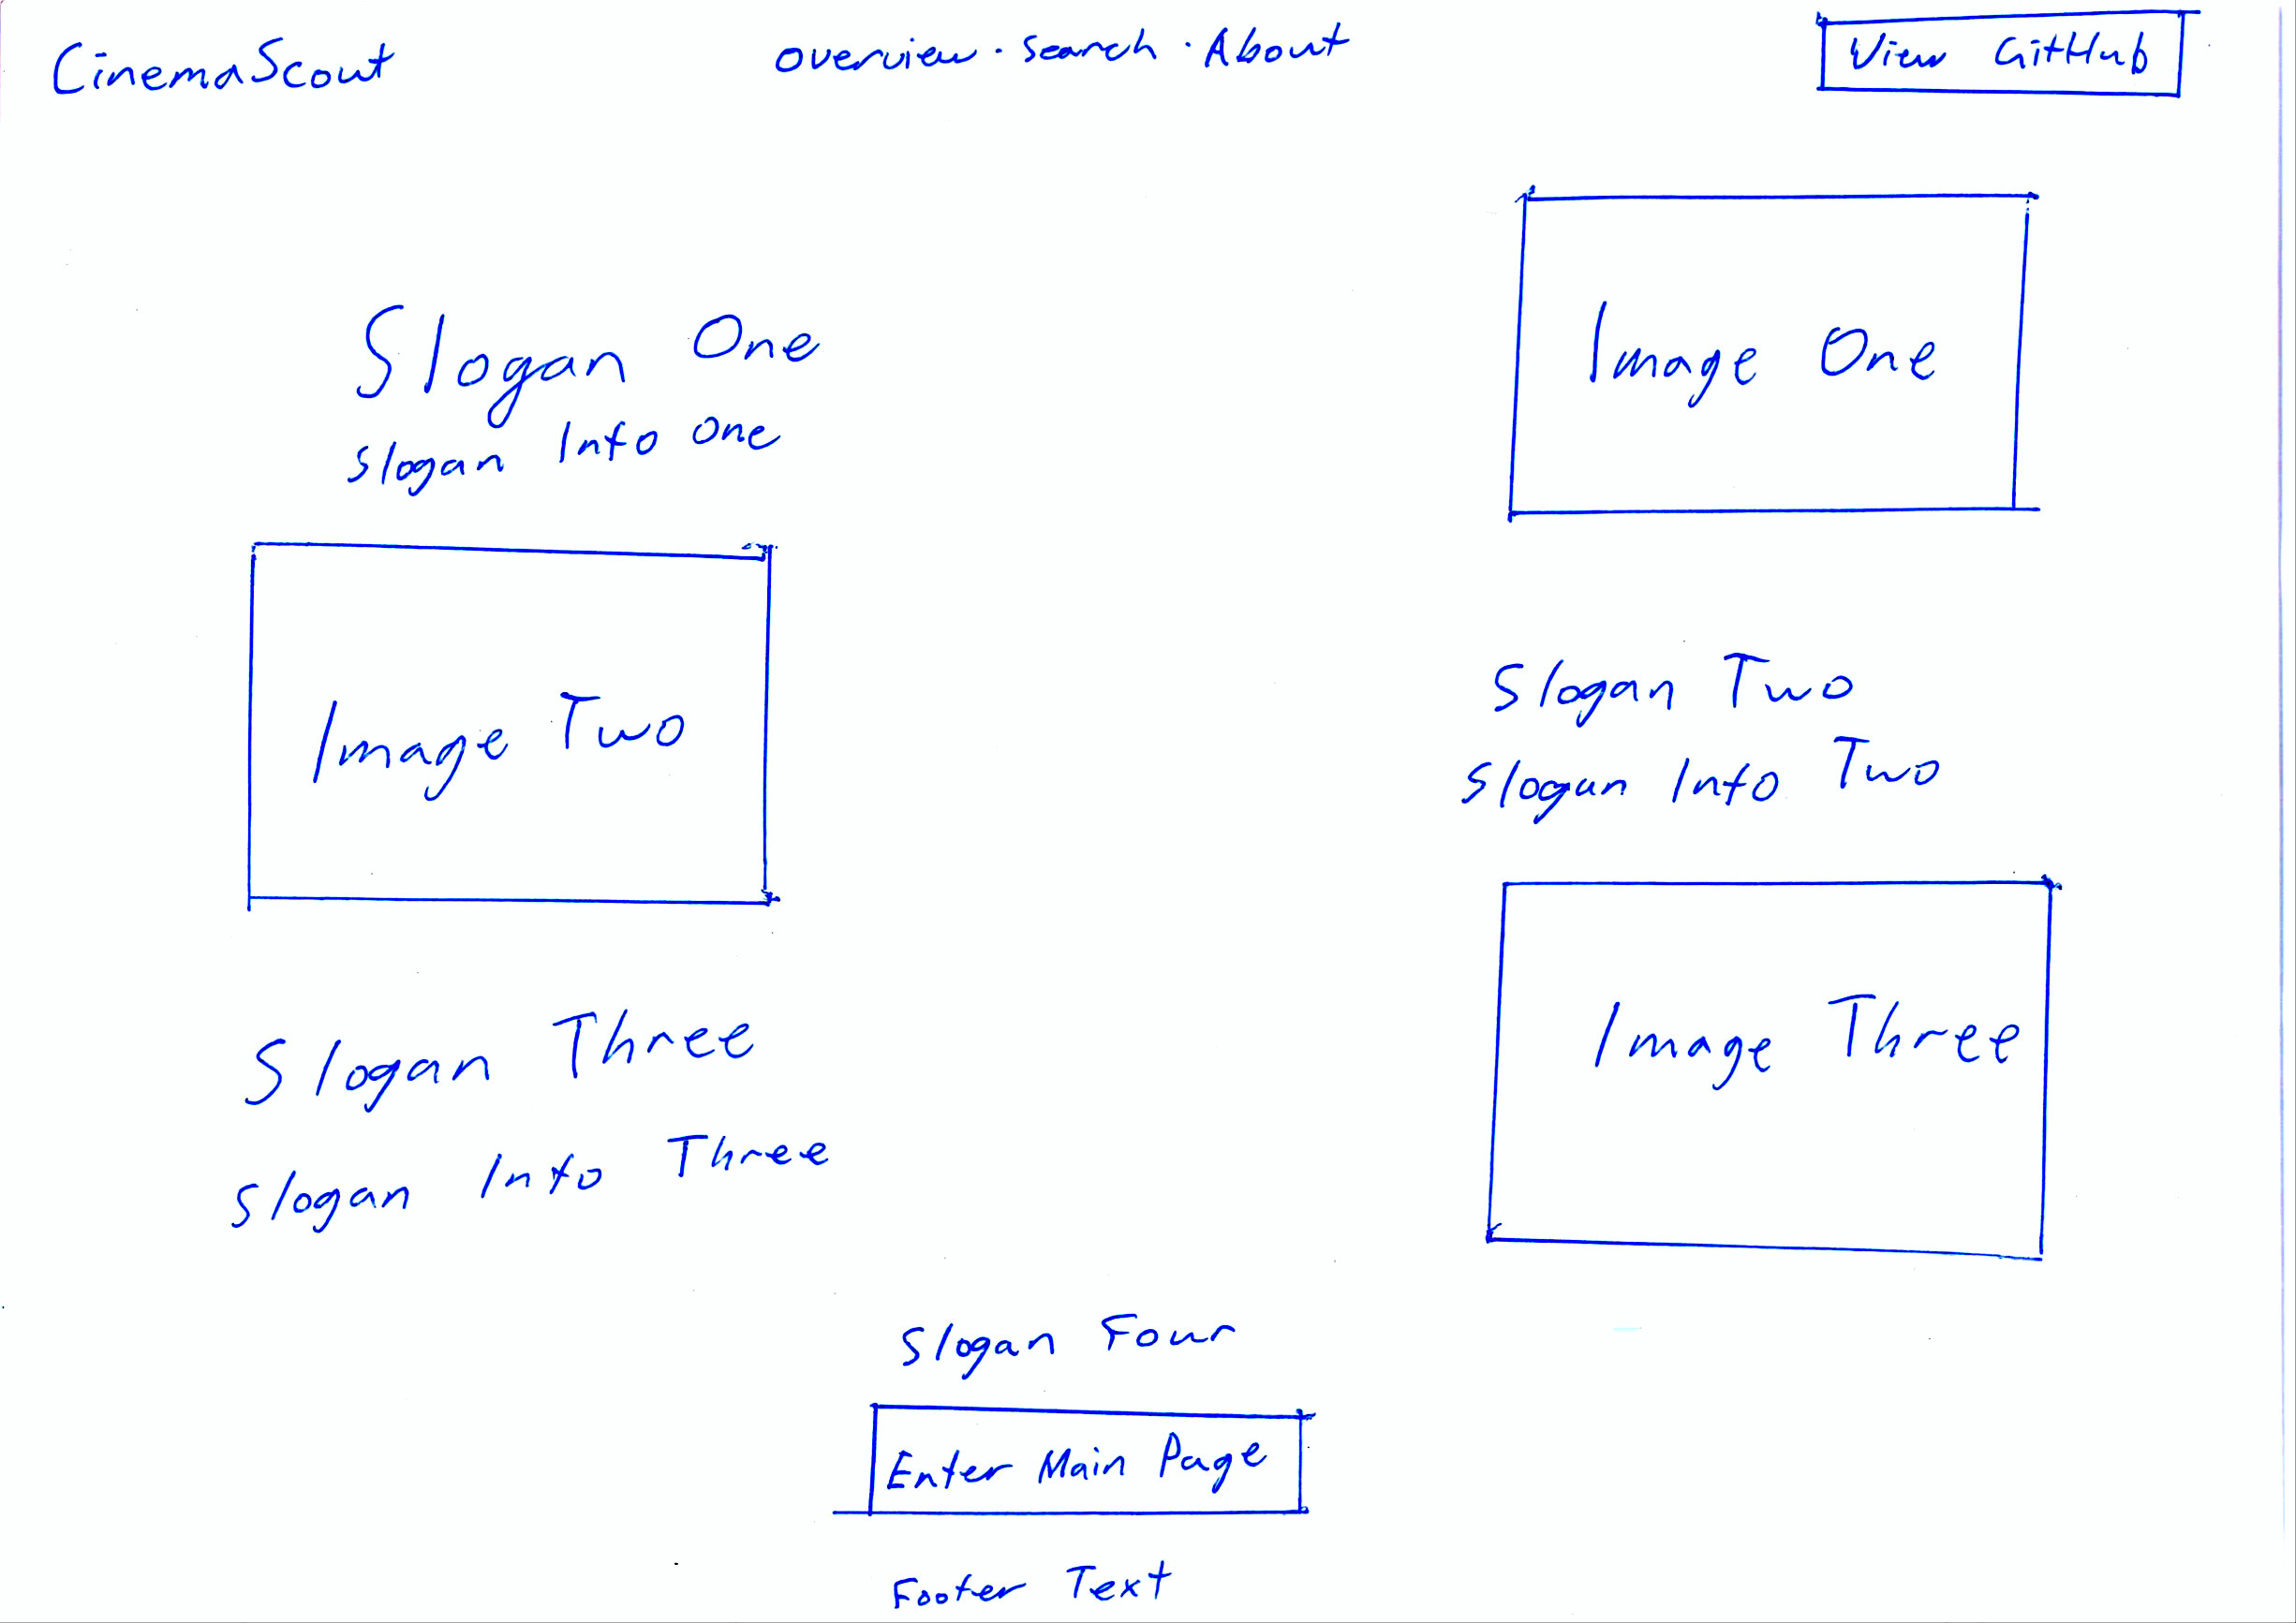
\includegraphics[width=\columnwidth]{res/landing.jpg}
\caption{Rough sketch of the landing page.}
\end{figure}
\subsection{Search Page}
\begin{figure}[H]
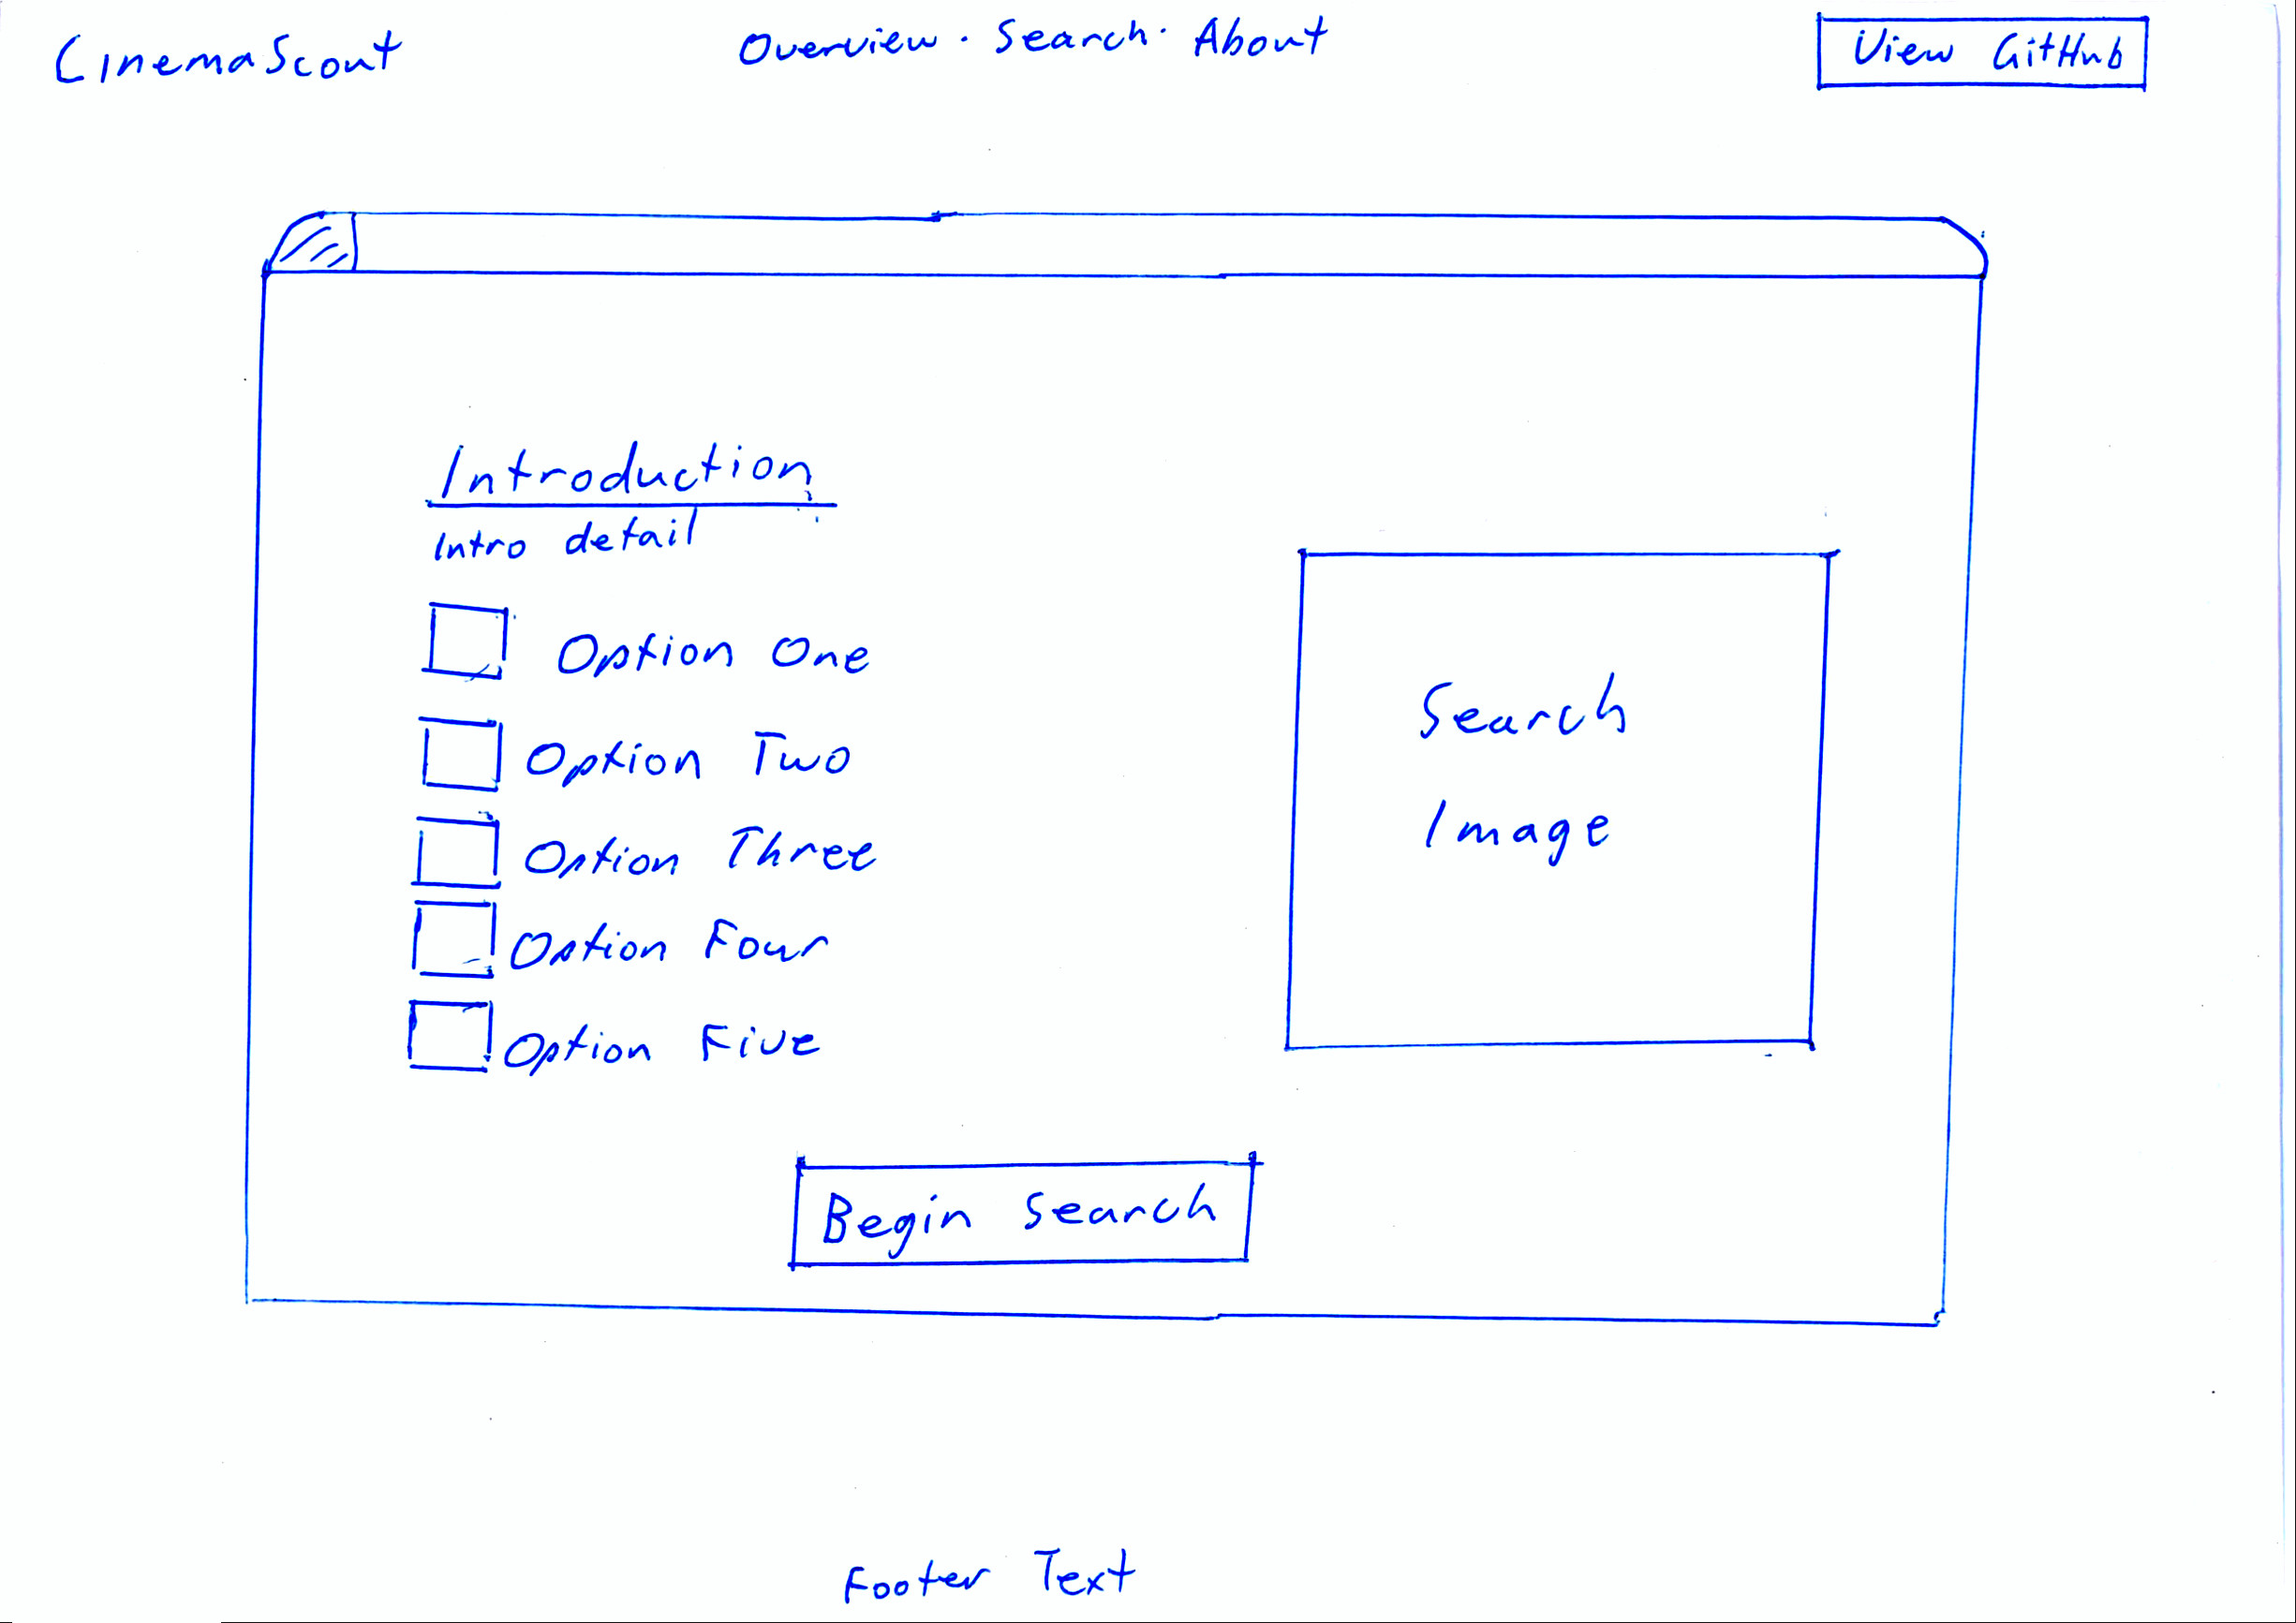
\includegraphics[width=\columnwidth]{res/search_begin.jpg}
\caption{Rough sketch of the initialise search state of the search page.}
\end{figure}
\begin{figure}[H]
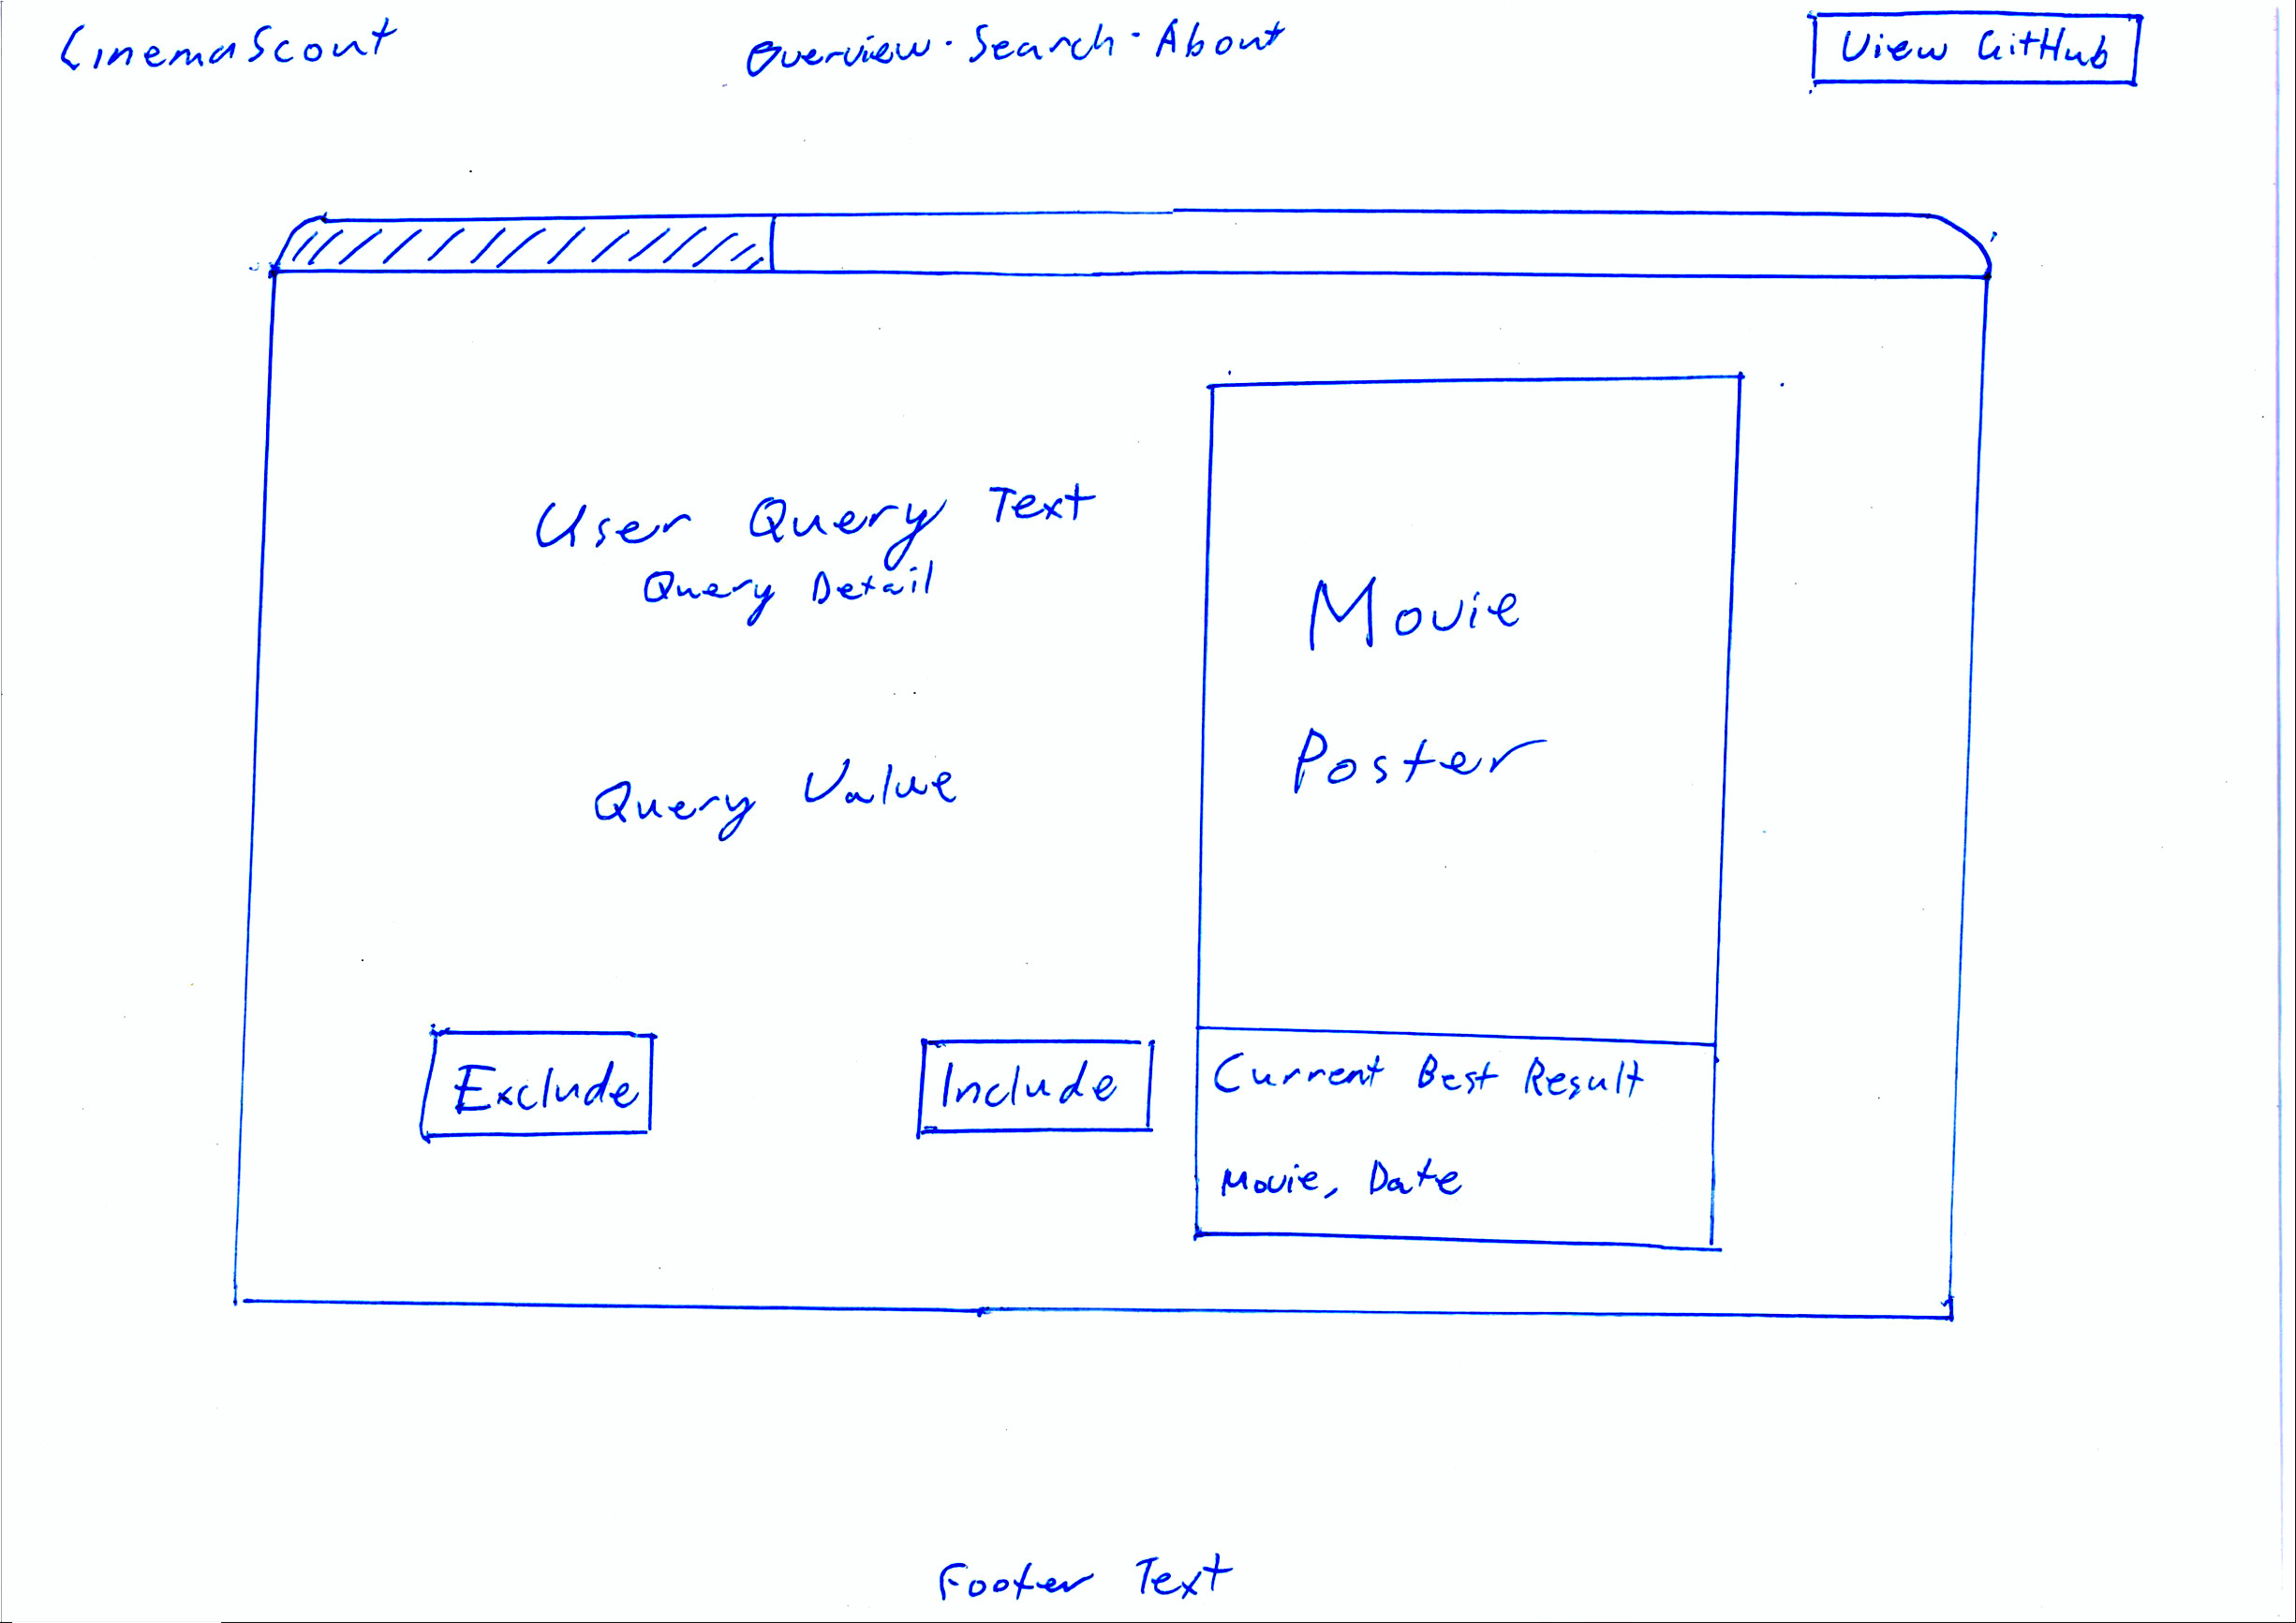
\includegraphics[width=\columnwidth]{res/search_next.jpg}
\caption{Rough sketch of the in progress state of the search page.}
\end{figure}
\subsection{About Page}
\begin{figure}[H]
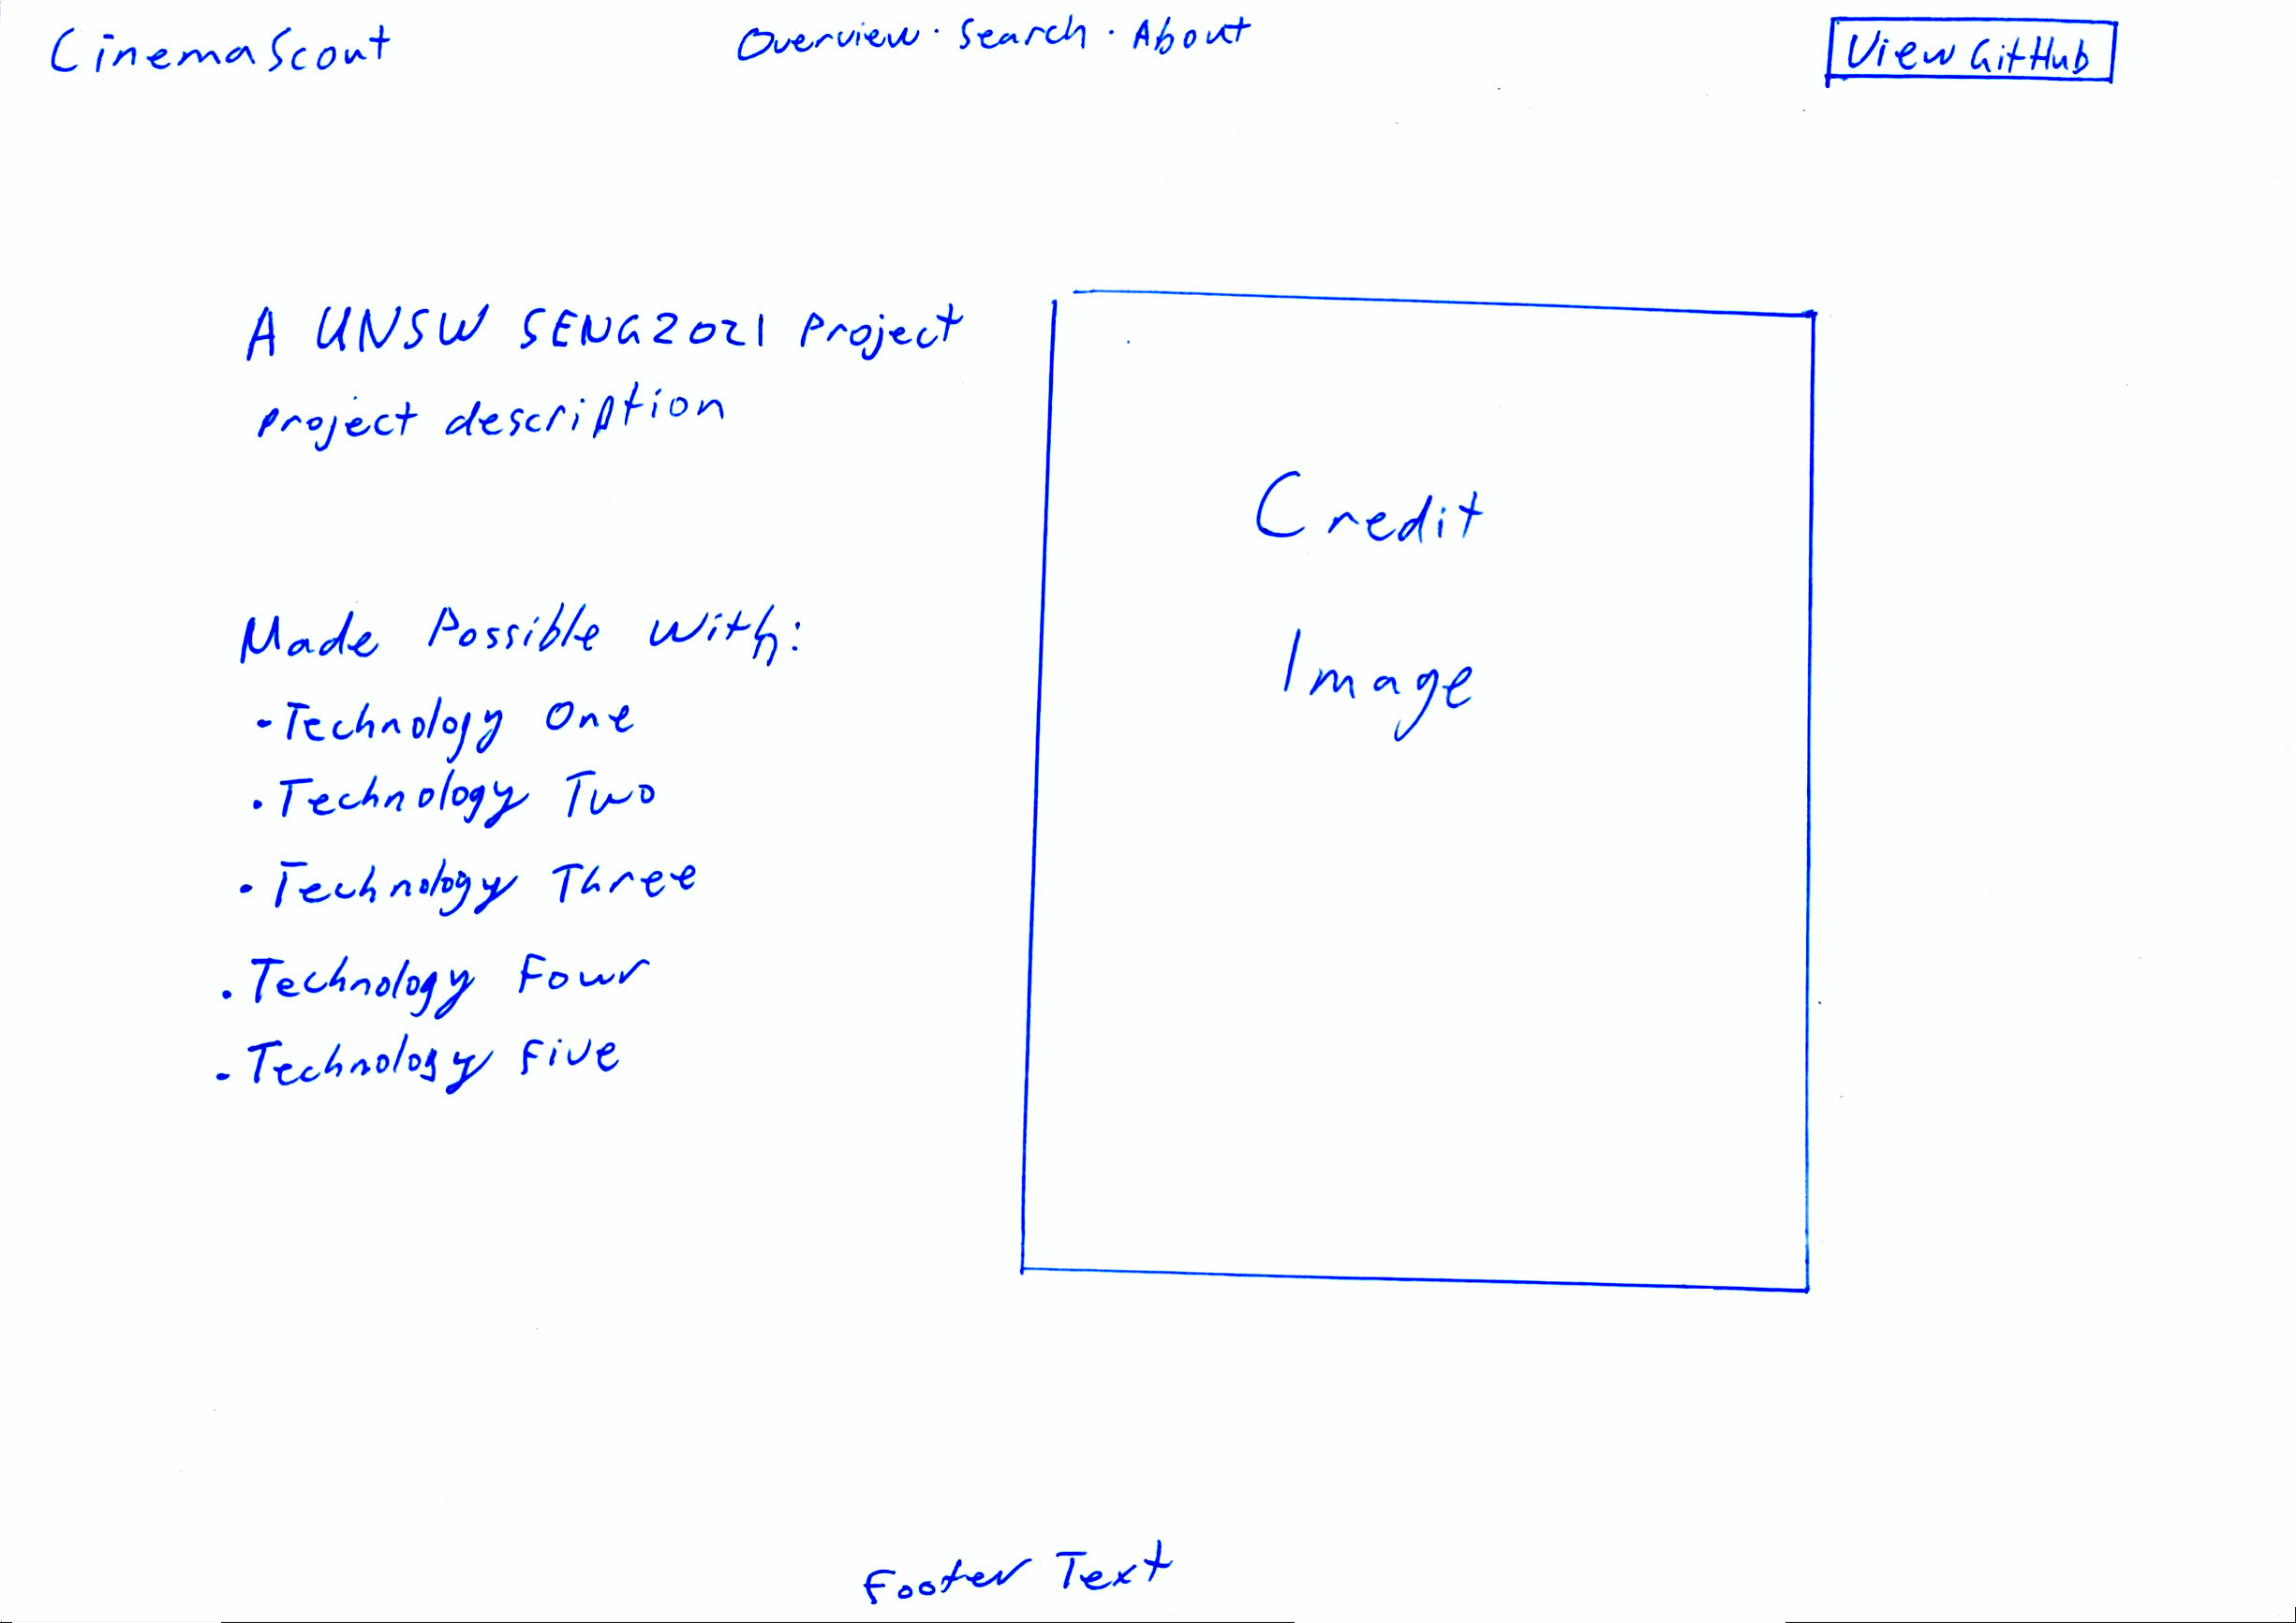
\includegraphics[width=\columnwidth]{res/credits.jpg}
\caption{Rough sketch of the about page.}
\end{figure}
\subsection{Storyboard Composite}
As an alternative to the traditional arrows used in storyboards and due to the
complexity of the user interface, we have instead represented each page
chronologically in appearance to a user and used colour to represent links
to other pages.
\begin{figure}[H]
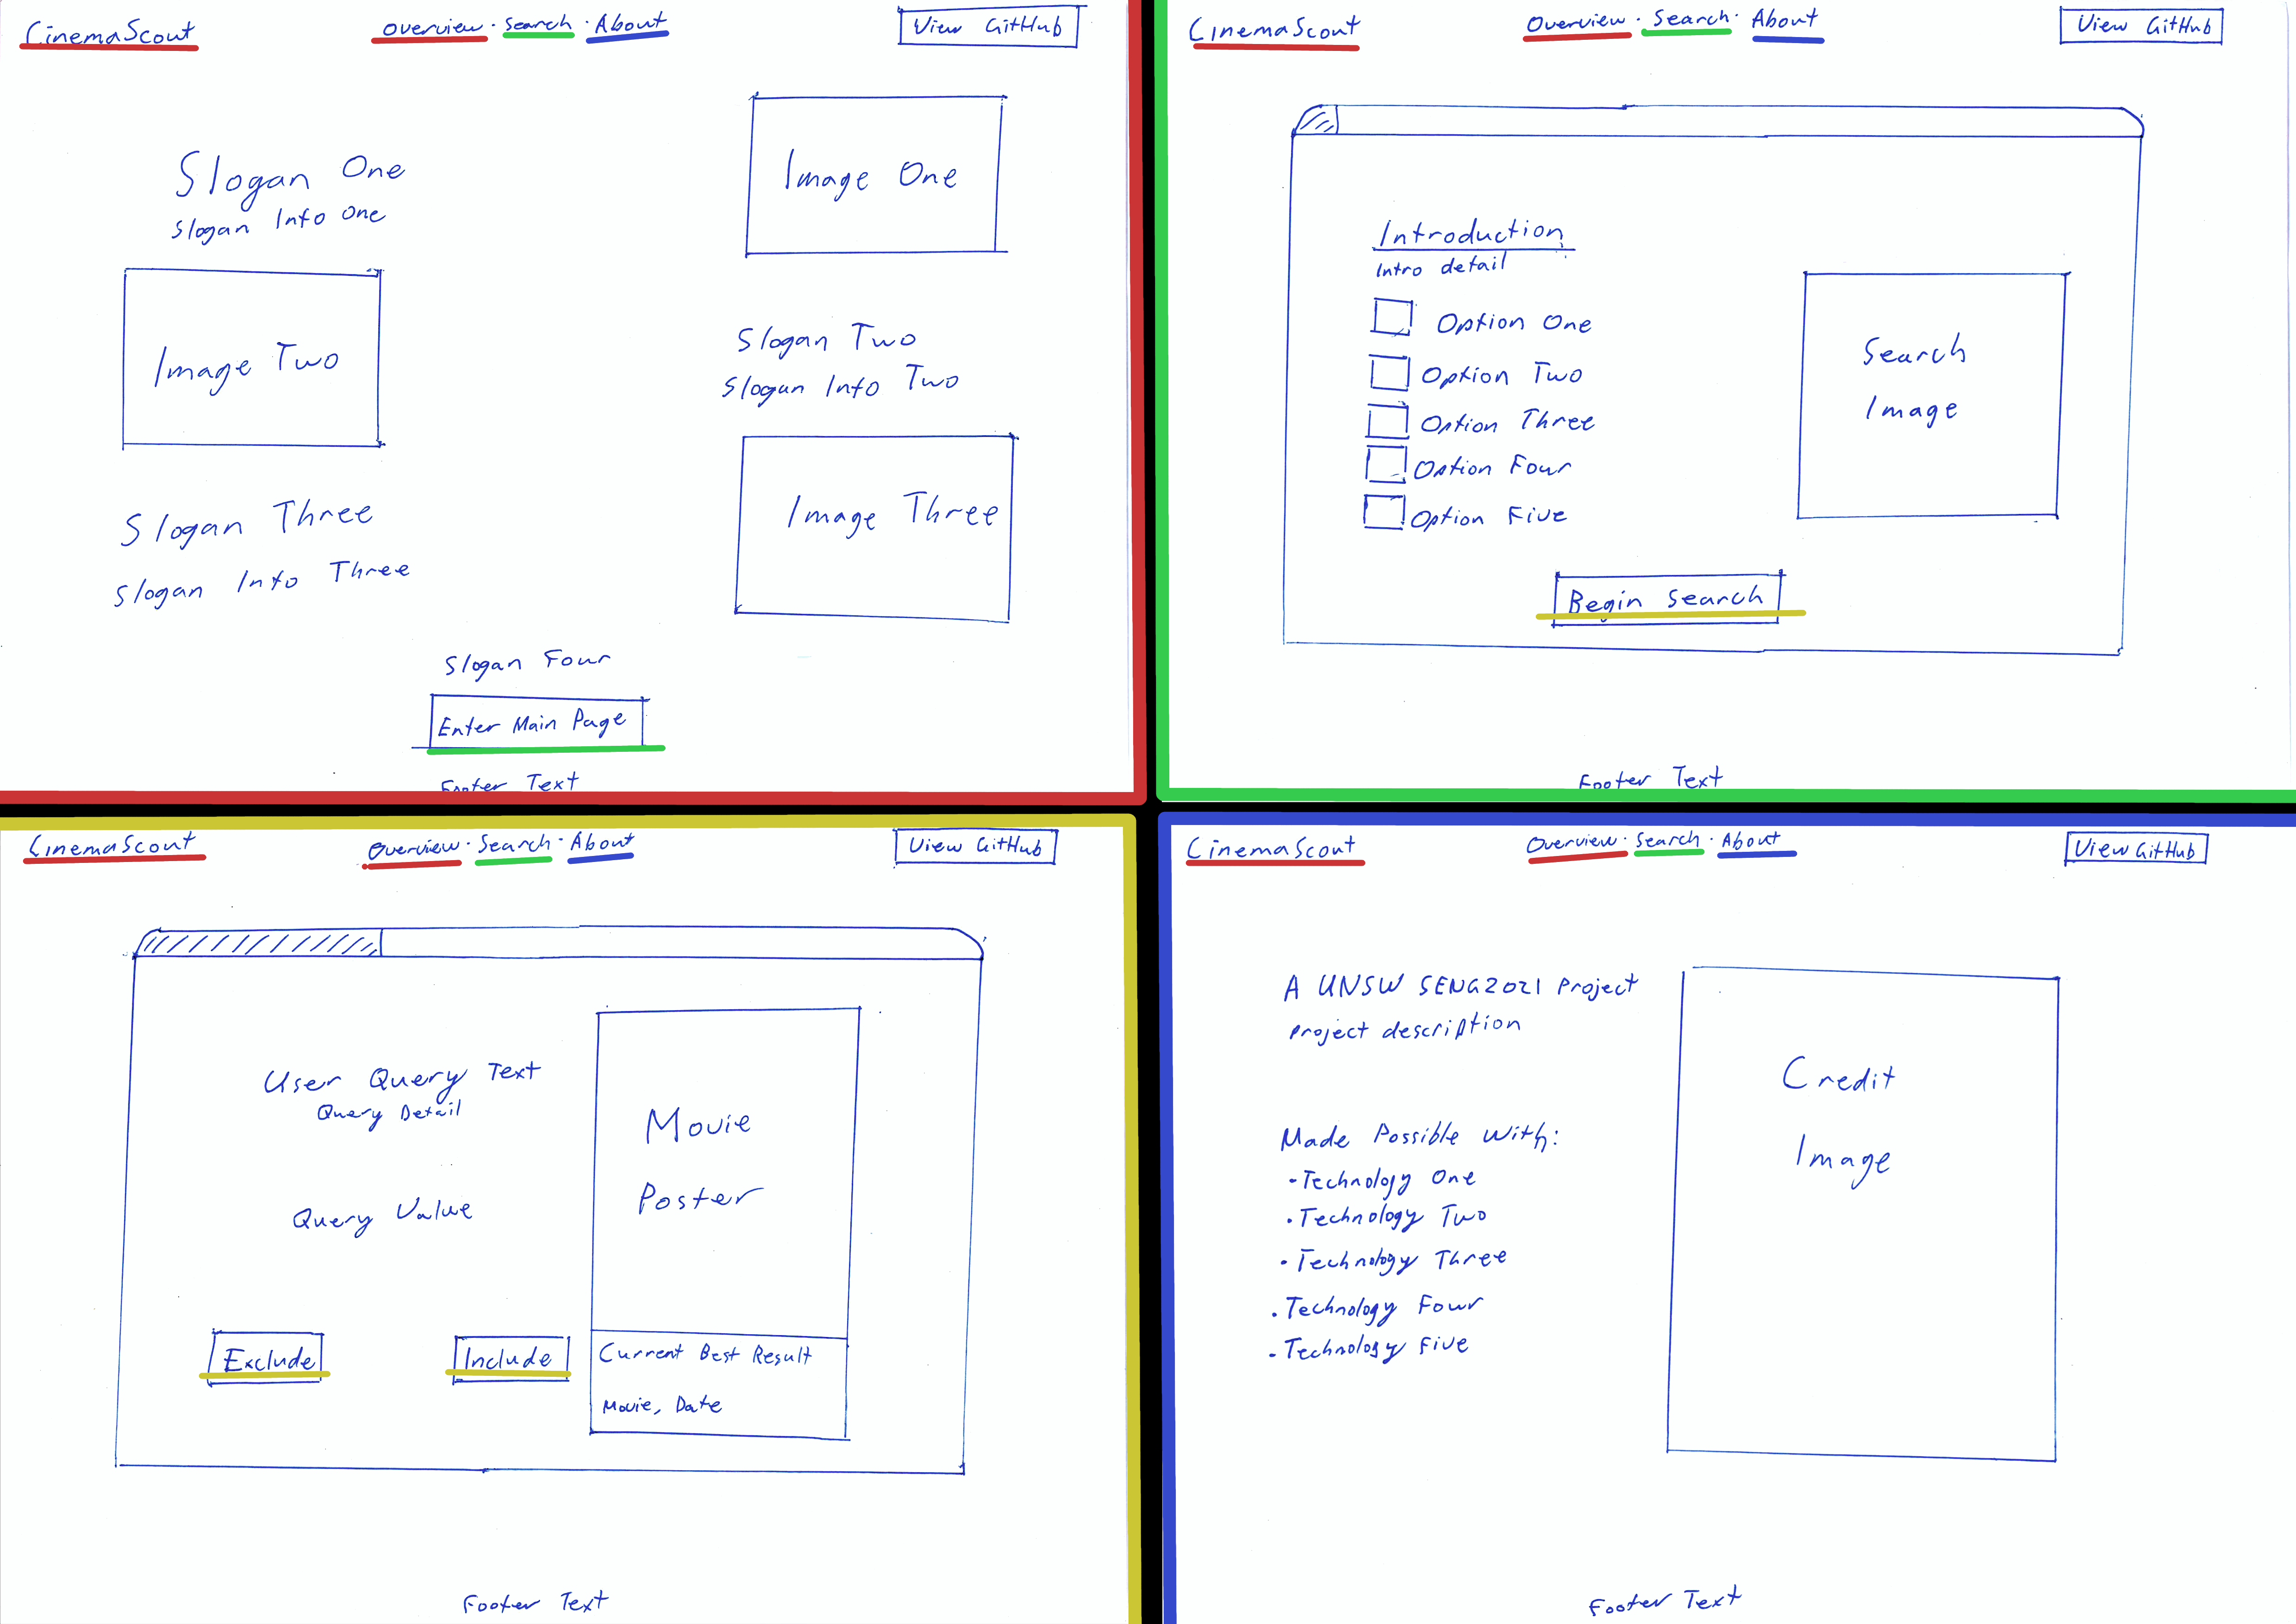
\includegraphics[width=\columnwidth]{res/arrows.png}
\caption{Storyboard sketch of all previous figures.}
\end{figure}

\section{High-Fiedelity Prototype}
The following images are a work in progress and do not represent the final
design of the product. All images were captured at a resolution of 1920 x
1080 using a default Chromium browser on Arch Linux.
\subsection{Landing Page}
\begin{figure}[H]
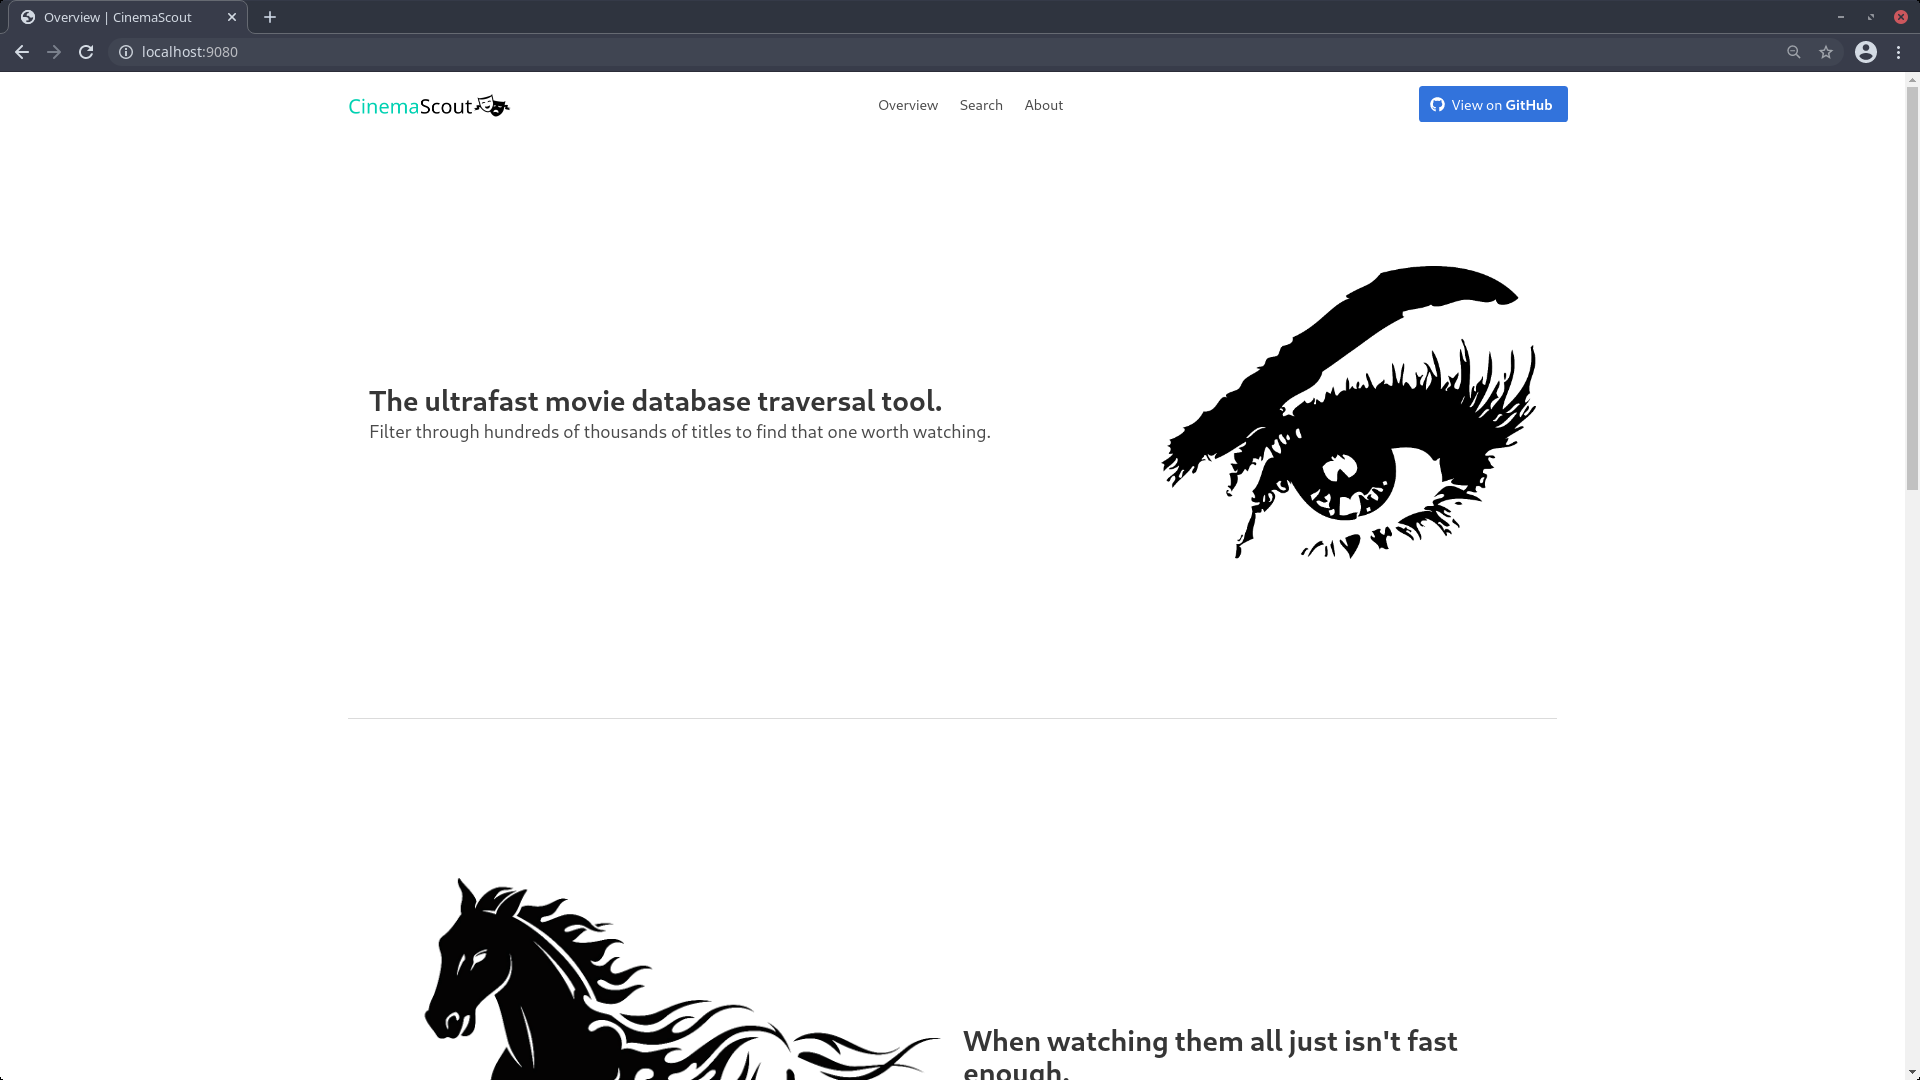
\includegraphics[width=\columnwidth]{res/landing_1.png}
\caption{Upper portion of the landing page.}
\end{figure}
\begin{figure}[H]
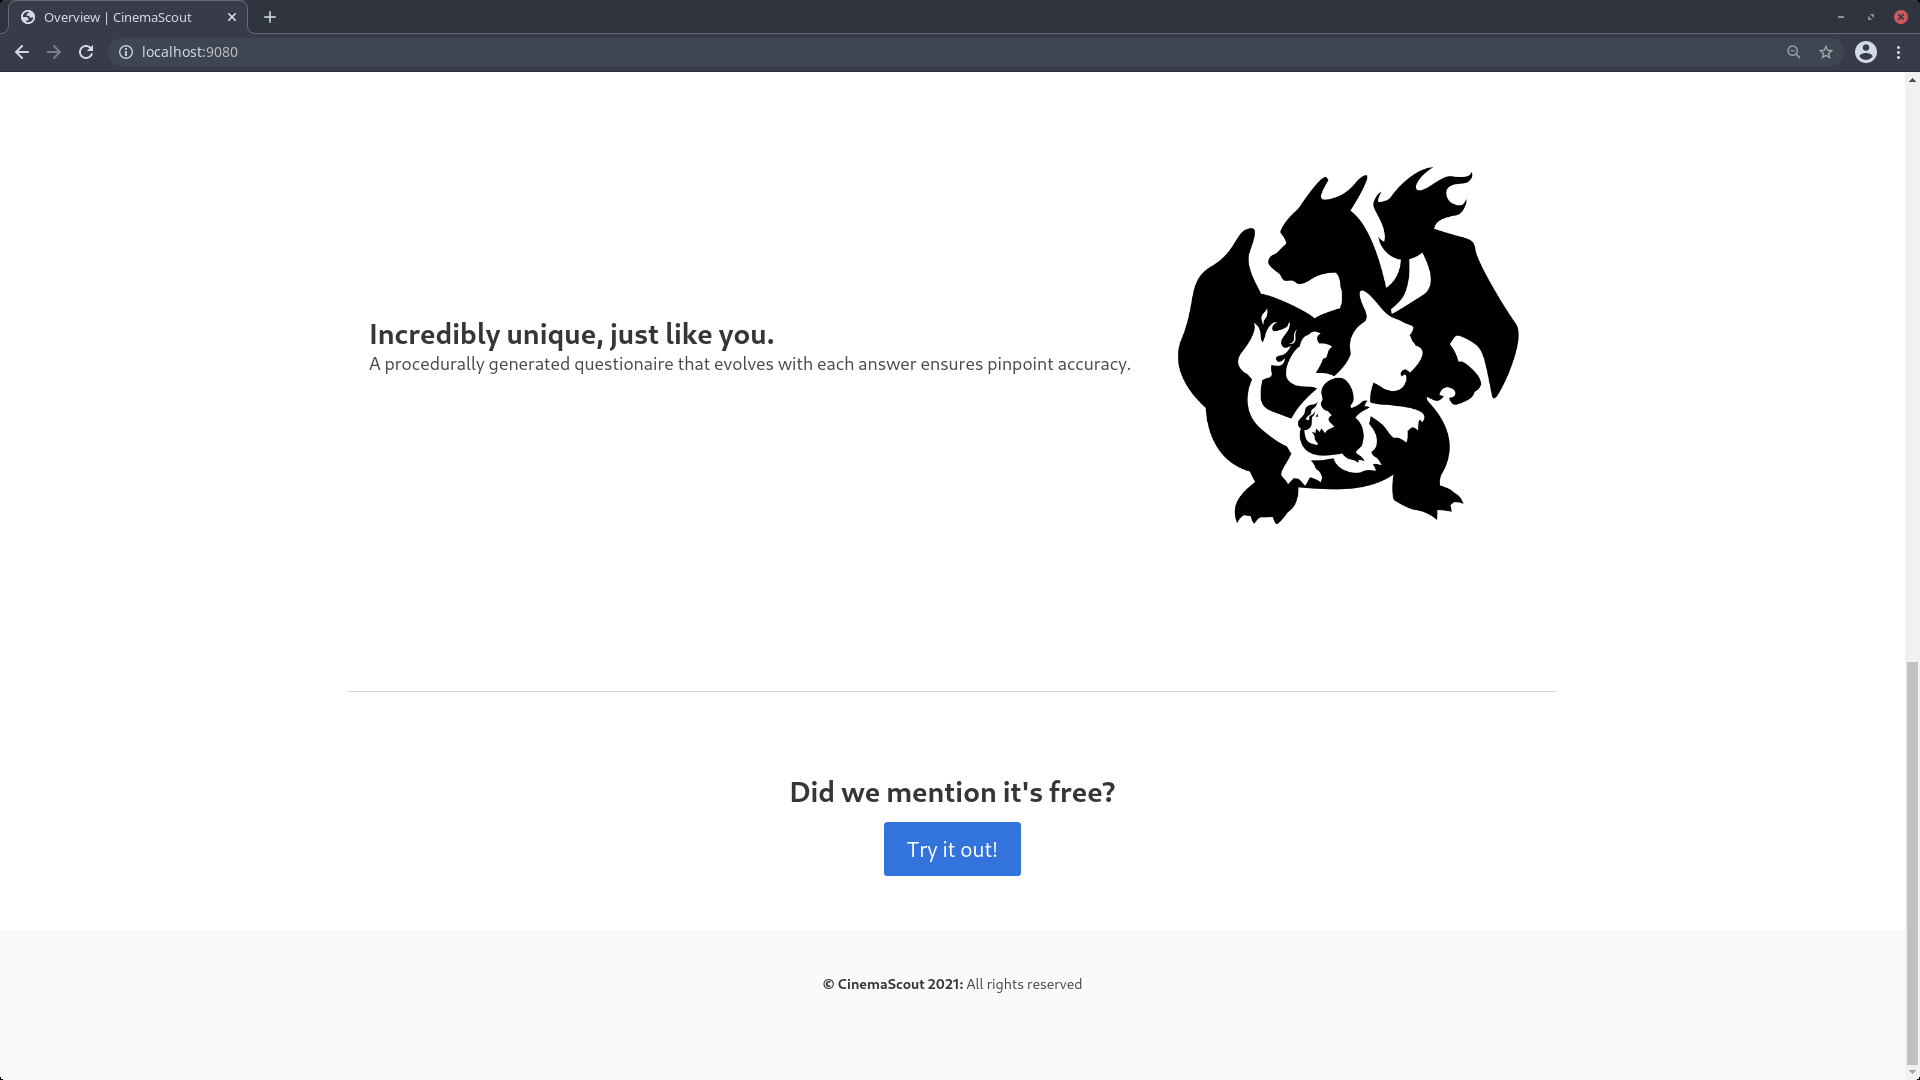
\includegraphics[width=\columnwidth]{res/landing_2.png}
\caption{Lower portion of the landing page.}
\end{figure}
\subsection{Search Page}
\begin{figure}[H]
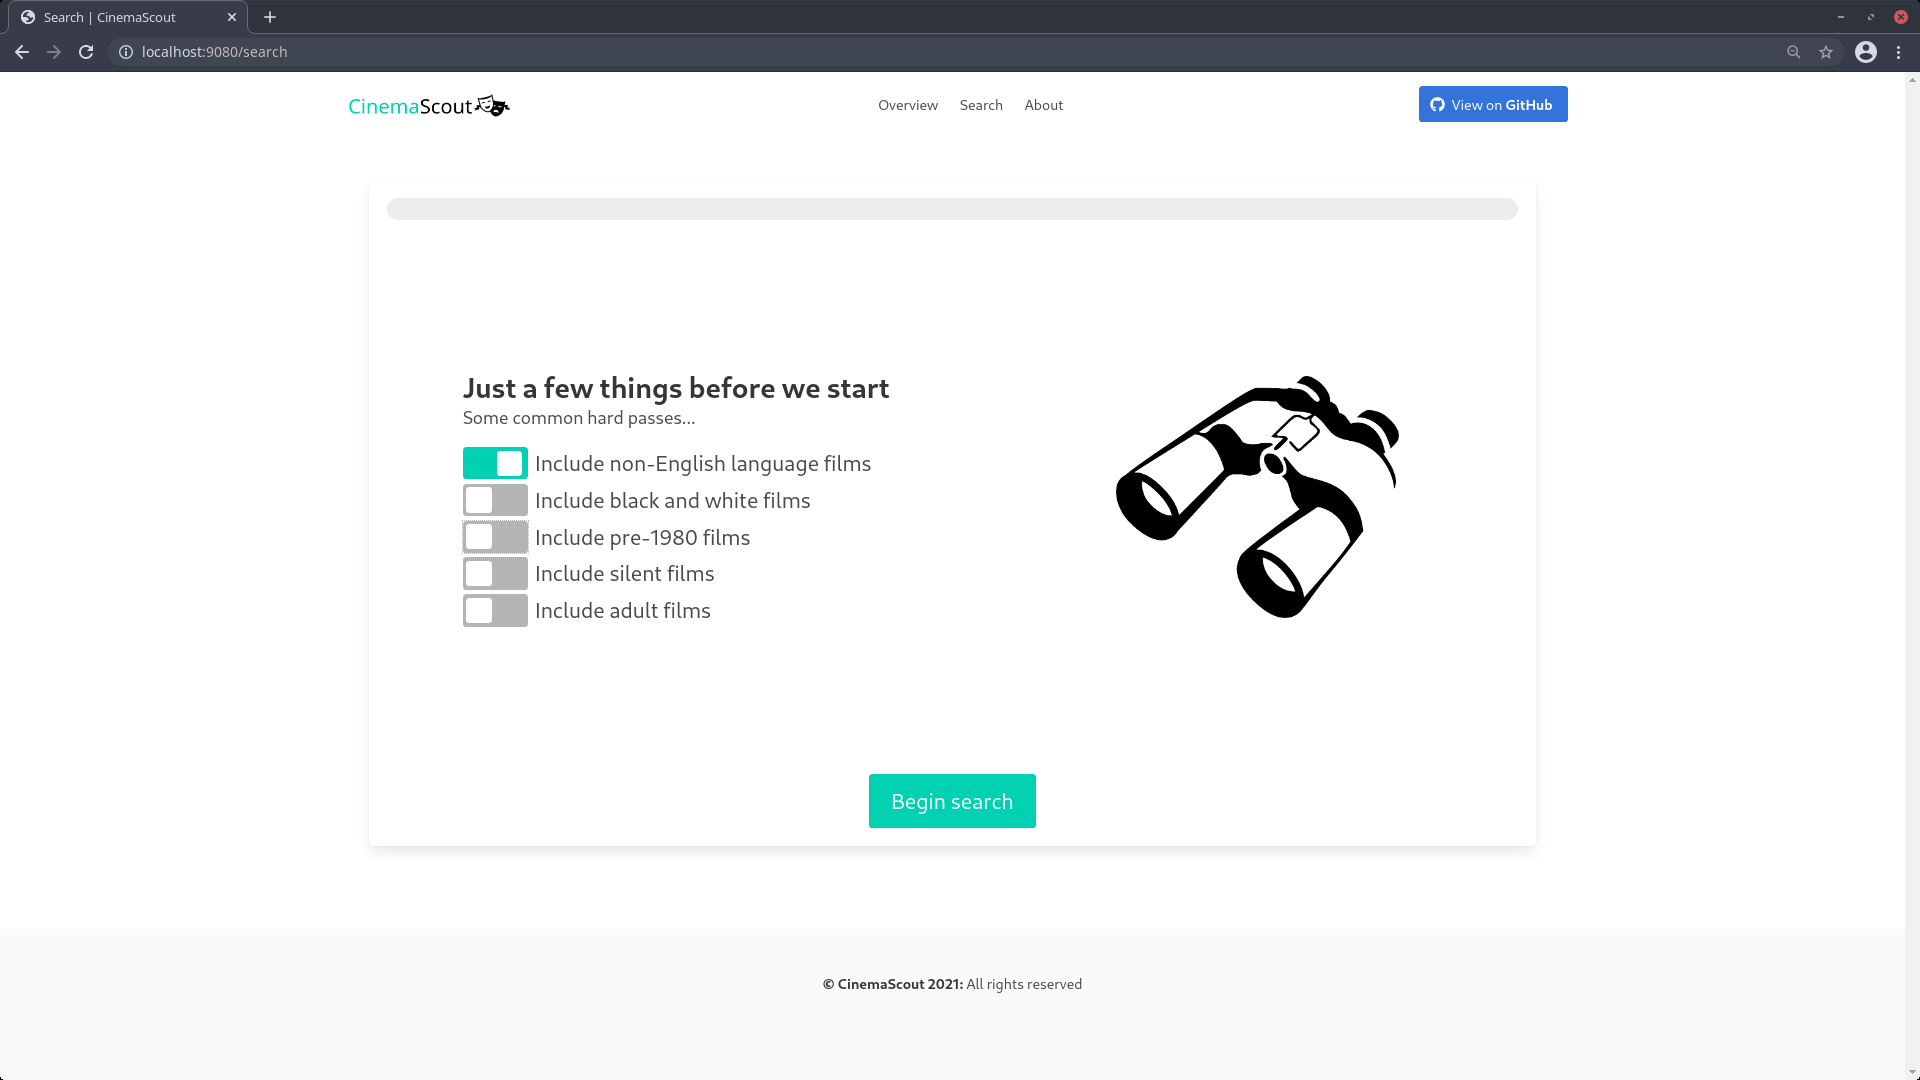
\includegraphics[width=\columnwidth]{res/search_1.png}
\caption{Initialise search state of the search page.}
\end{figure}
\begin{figure}[H]
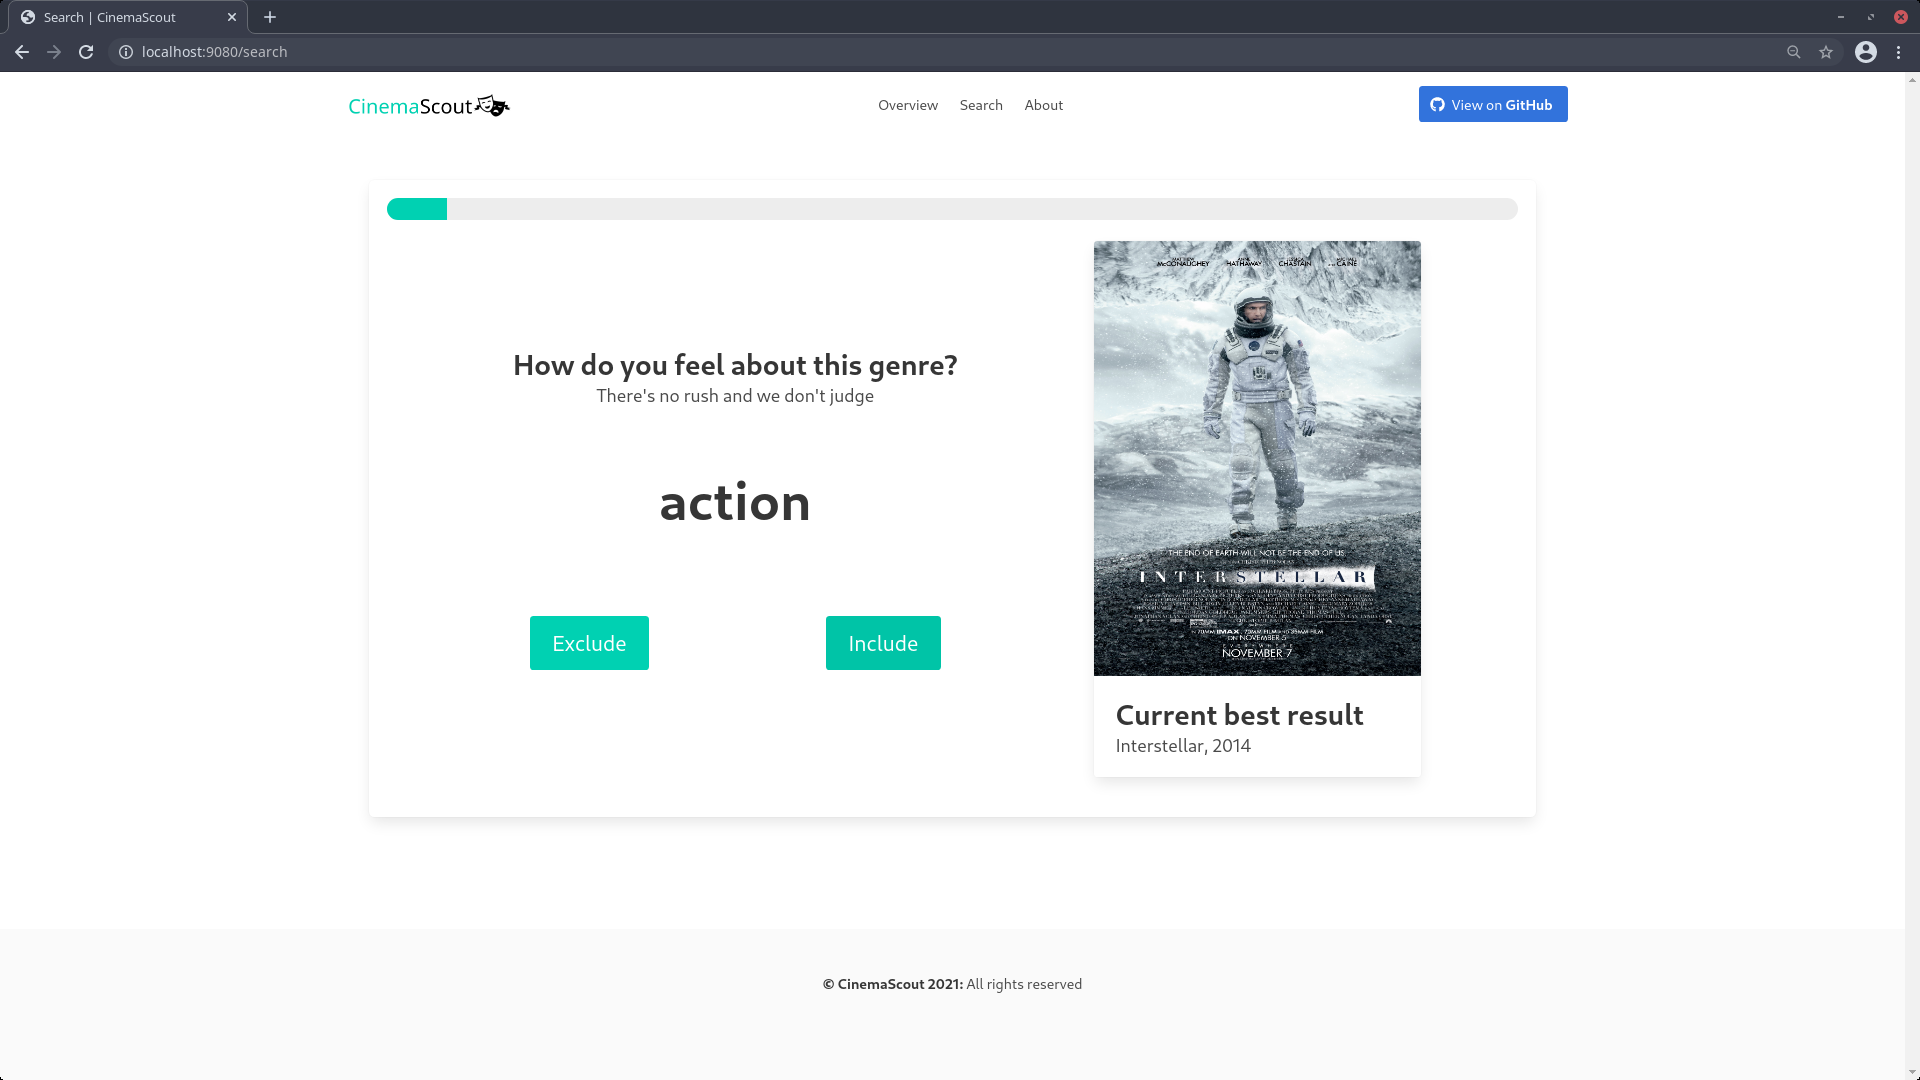
\includegraphics[width=\columnwidth]{res/search_2.png}
\caption{Search in progress state of the search page.}
\end{figure}
\subsection{About Page}
\begin{figure}[H]
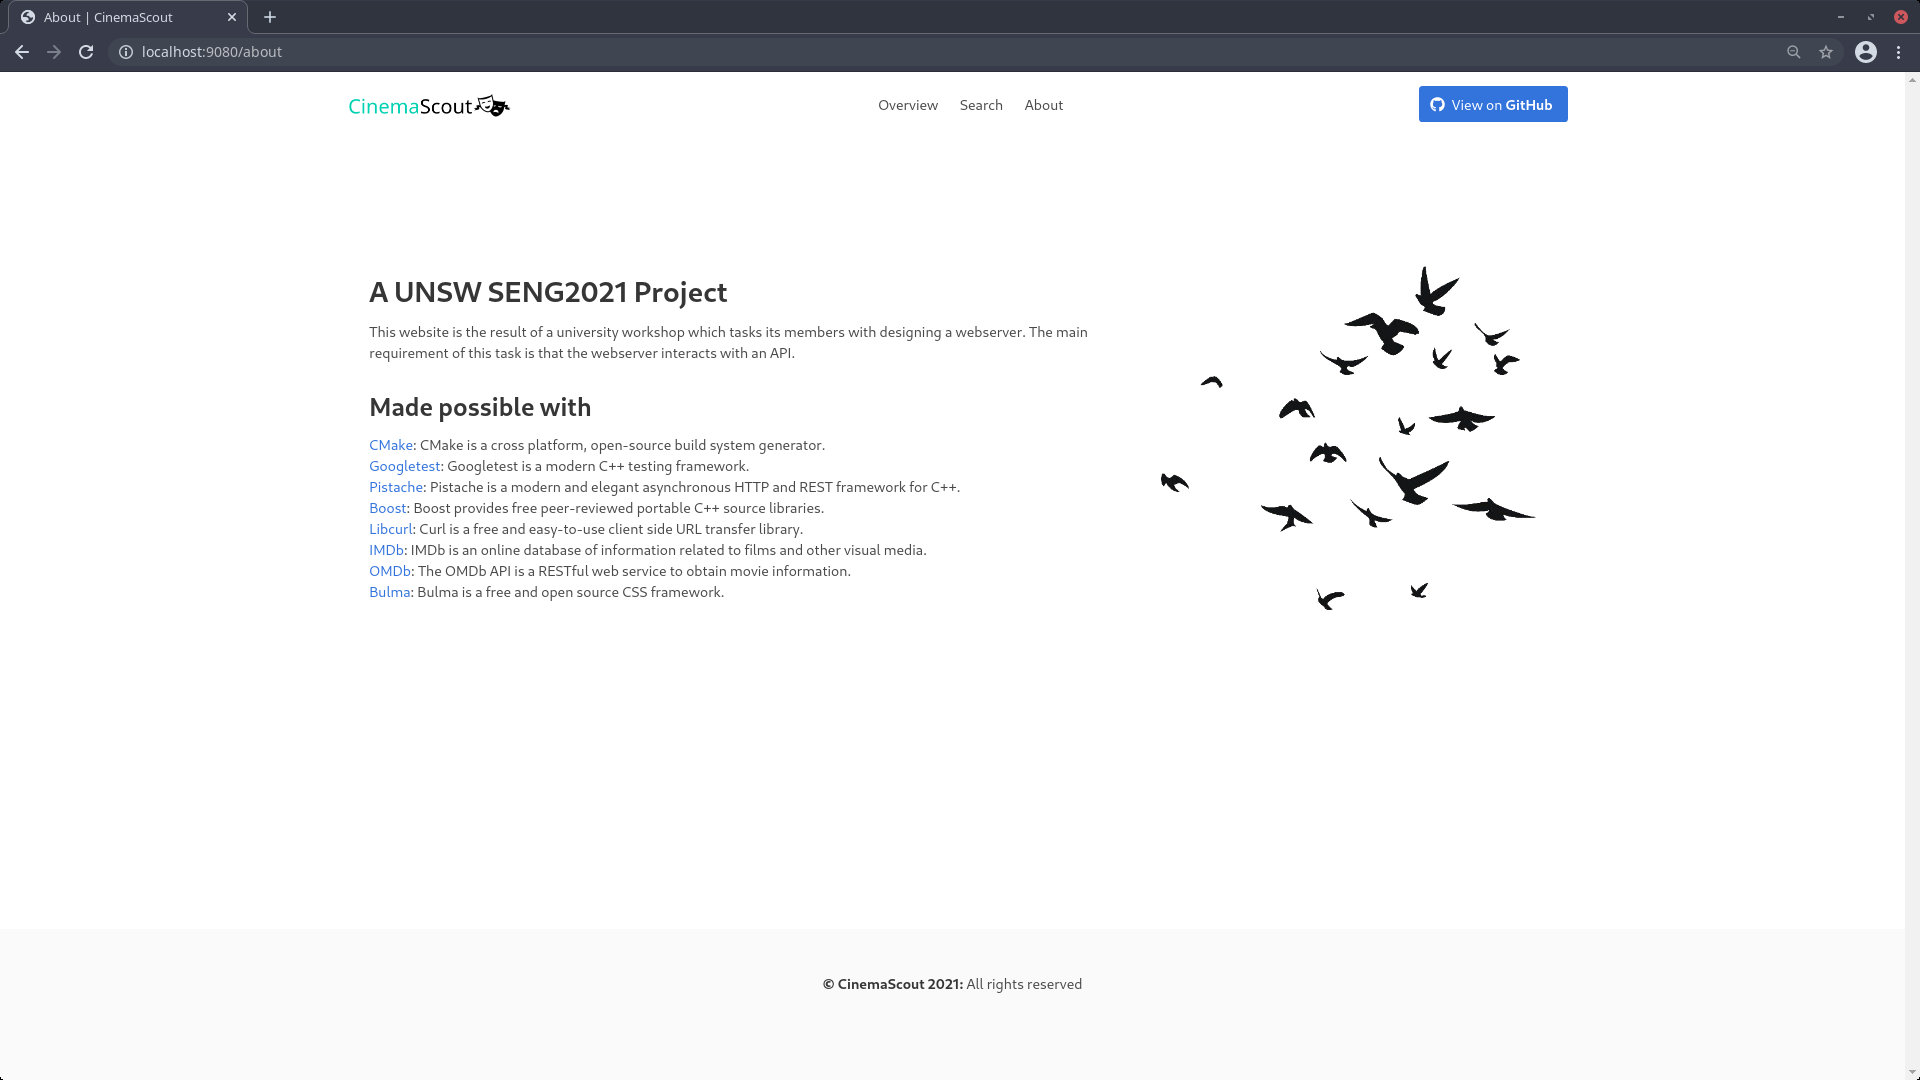
\includegraphics[width=\columnwidth]{res/about.png}
\caption{Entire portion of the about page.}
\end{figure}

\end{document}
